\chapter{Совместное использование сильно и слабо размеченных наборов данных} \label{chapt3}

\section{Мотивация} \label{sect3_1}

Как было сказано в предыдущей главе, классический MIL имеет ряд ограничний в том числе на размер карты. Поэтому были сформулированы следущие задачи:

\begin{itemize}
    \item Создать систему, которая способна возвращать карты сегментации более высокого разрешения;
    \item Оснастить данную систему возможностью обучаться как на сильно так и на слабо размеченных наборах данных;
\end{itemize}

\noindent При решении даннных задач было обращено внимание на \cite{retinopathy}, где авторы уже решали подобную задачу. Они предложили пирамидальную интегральную структуру слоёв нейросети, которая один за одним последовательно суммирует с различными коэффициентами значения слоёв сети, с каждым шагом увеличивая размерность. В результате ряда экспериментов, мы остановились на архитектуре, изображенной на рис. \ref{fig:schema_total}. При этом предлагается следующий порядок обучения системы(рис. \ref{fig:schema_order}):

\begin{figure}[h] 
  \center
  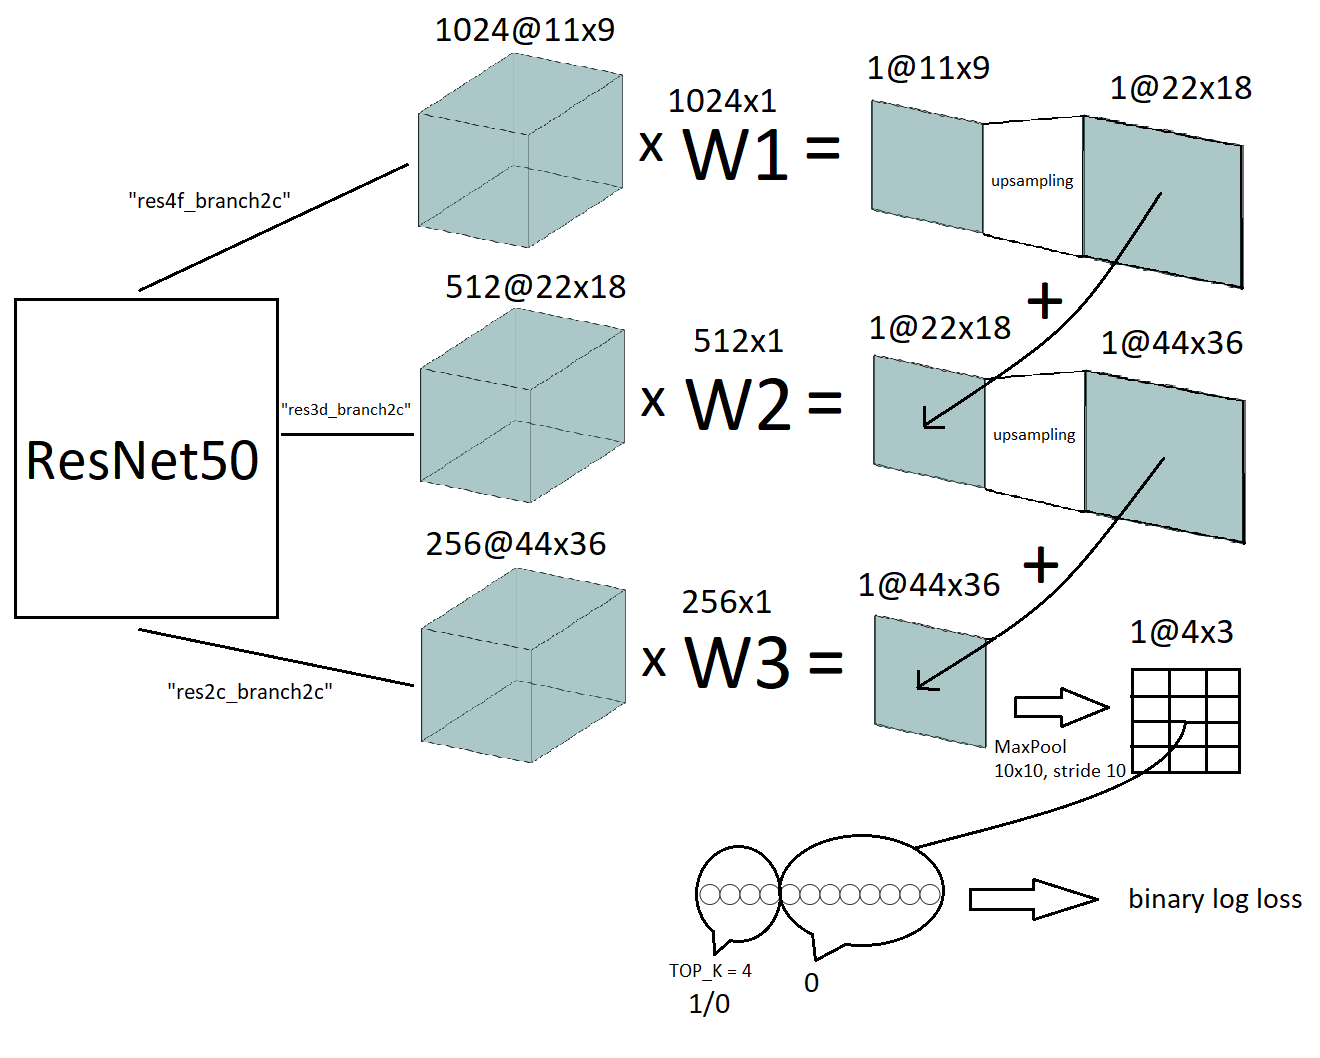
\includegraphics [scale=0.64] {images/schema_total.png}
  \caption{Схема архитектуры} 
  \label{fig:schema_total}  
\end{figure}


\begin{figure}[h] 
  \center
  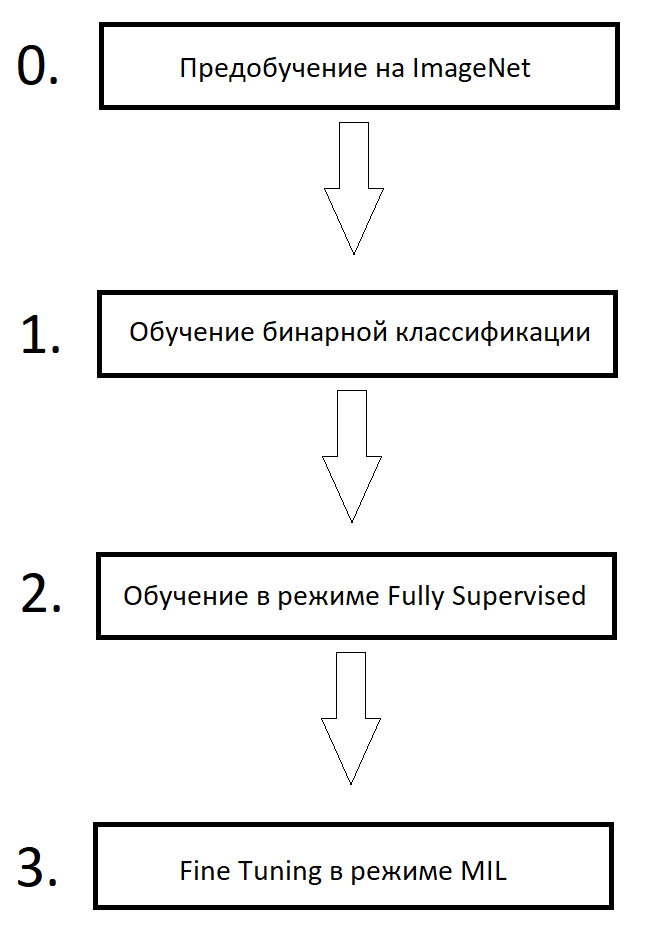
\includegraphics [scale=0.6] {images/schema.png}
  \caption{Порядок обучения} 
  \label{fig:schema_order}  
\end{figure}


\begin{enumerate}[start=0]
    \item Инициализация весов ResNet-50 весами после предобучения на ImageNet позволяет ускорить дообучение геометрических признаков, так как часть геометрических конфигураций уже <<усвоена>> сетью;
    \item Данный пункт будет изучен ниже. Выдвигается гипотеза, что, поскольку, распределение данных на ImageNet сильно отличается от распределения медицинских изображений, то имеет смысл сперва обучить классификацию, чтоб сеть <<адаптировала>> извлекаемые признаки под новое распределение, а затем переходить к обучению сегментации;  
    \item Далее идёт обучение сегментации на карте 44x36 с использованием сильной разметки на сильно размеченном наборе данных(малая часть данных);
    \item После этого предлагается улучшить полученную сегментацию путём применения метода MIL;
\end{enumerate}

На рис.\ref{fig:arch_class} изображена использованная архитектура модели классификации. Модели для всех трёх описанных видов обучения построены на основе {\bf одной и той же} модели ResNet-50 и имеют {\bf общие} слои с разделяемыми коэффициентами.

\begin{figure}[h] 
  \center
  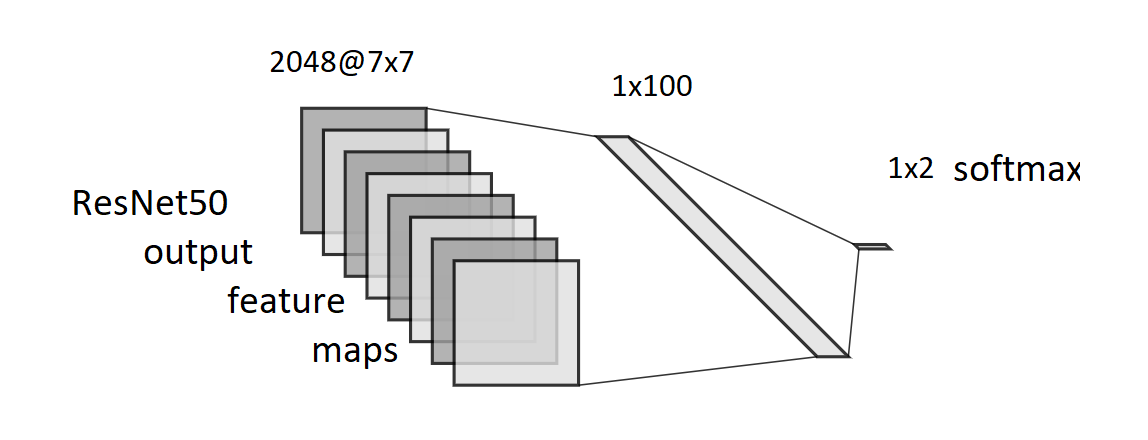
\includegraphics [scale=0.6] {images/arch_class.png}
  \caption{Архитектура модели классификации} 
  \label{fig:arch_class}  
\end{figure}



В последующих разделах будет обсуждаться подбор параметров системы и параметров обучения, предложенный порядок обучения(рис.\ref{fig:schema_order}), в частности, порядок следования пп.3 и 4, а также будут приведены численные результаты экспериментов с учётом кросс-валидации.

\section{Данные}

Для разработки системы сегментации нами были использованы данные конкурса по сегментации новообразований в мозге BRATS2018. Данный набор данных содержит 285 пациентов с диагнозом глиома. Для каждого пациента предоставлен набор слоёв МРТ в аксиальной проекции. Для каждого слоя дана попиксельная разметка опухоли, если она представлена в данном сечении. Сегментированная опухоль также разделена на несколько составных частей, однако мы в своей работе используем сегментацию опухоли целиком("whole tumor" на изображении ниже \ref{fig:bratss}).  Томографические снимки могут исполняться в различных контрастах. В наших экспериментах был использован контраст T1Gd. 

\begin{figure}[ht] 
  \center
  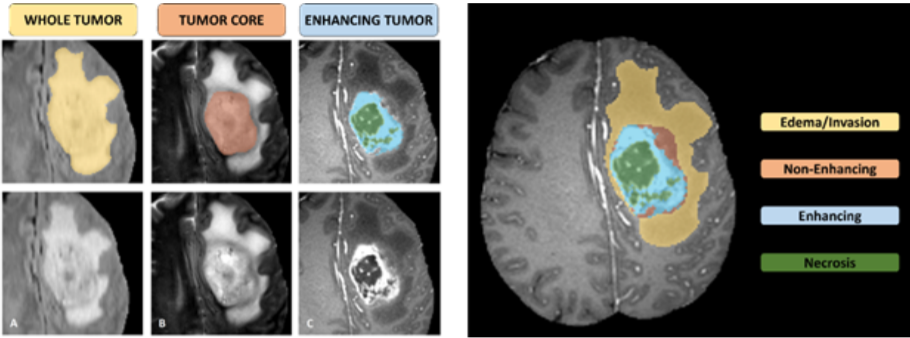
\includegraphics [scale=0.6] {images/brats.png}
  \caption{ Пример изображения мозга с сегментацией новообразования и его составных частей} 
  \label{fig:bratss}  
\end{figure}
Поскольку проекции мозга имеют различную площадь, крайние сечения могут быть существенно малы в сравнении с центральными сечениями. По этой причине крайние сечения, имеющие зачастую отличающуюся от средних сечений форму, были выброшены из рассмотрения. Всего число отобранных снимков для отдельно взятого пациента варьируется от 98 до 123 и в среднем составляет {\bf 110}. Соотношение числа снимков, содержащих опухоль, к снимкам, ее не содержащим, варьируется от 0.22 до 9.18 и в среднем составляет {\bf 1.25}. Общее число изображений составляет {\bf 31350}, в т.ч. 15761 снимков, содержащих опухоль. 

Для каждого пациента серия снимков была выровнена таким образом, чтоб минимизировать фоновую площадь изображения(см. \ref{fig:transform}). Затем все изображения были приведены к формату 170x140.

\begin{figure}[ht] 
  \center
  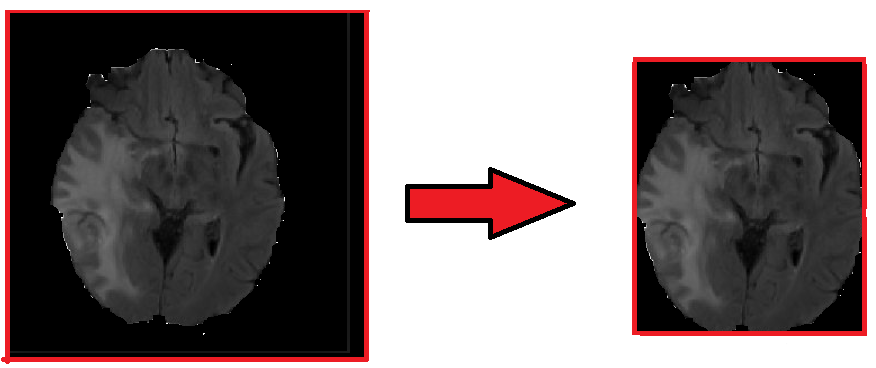
\includegraphics [scale=0.6] {images/transform.png}
  \caption{ Пример выравнивания серии изображений по крайним для нее достижимым границам изображения} 
  \label{fig:transform}  
\end{figure}

С целью упрощения реализации задач данной ранной работы на даннном этапе при выборе слоёв, содержащих опухоль, мы ограничились случаями, в которых опухоль занимает не менее 10\%, 5\% и 1\% от площади сечения {\bf мозга}(без фона) на изображении. Таким образом, были получены три набора данных:

\begin{center}
\begin{tabular}{||c |c ||} 
 \hline
  & Число изображений,  \\ [0.5ex]
  Выборка & содержащих опухоль \\
 \hline\hline
 \ge 10\% & 5636  \\ 
 \hline
 \ge 5\% & 9804 \\
 \hline
 \ge 1\% & 13806  \\[1ex] 
 \hline

 \hline
\end{tabular}
\end{center}
Впоследствии будет произведён анализ работы алгоритма на каждом из этих наборов данных.


\section{Метрика}

Прежде всего, следует определиться насчёт метрики для обучения на сильно размеченном наборе данных(fully supervised learning - будем обозначать {\bf FS}- обучение). 

Для задачи сегментации при обучении на данных с попиксельной разметкой обычно используют два вида метрик:
\begin{itemize}
    \item Индекс сходства Дайса(Dice index);
    \item Перекрестная энтропия(Binary crossentropy);
\end{itemize}

$$\text{Dice~index}(P,T) := \frac{2\sum_{i,j}P_{ij}T_{ij}}{\sum_{i,j}P^2_{i,j} + \sum_{i,j}T^2_{i,j}},$$
где P-пиксельная карта - предсказание($P_{i,j}\in [0,1]$), T - бинарная пиксельная карта($T_{i,j}\in\{0,1\}$). В качестве функции потерь при постановке задачи оптимизации метрики в терминах минимизации используют функцию потерь Дайса(Dice loss):

$$\text{Dice~loss} := 1 - \text{Dice~index}$$

Во избежание возможных проблем с делением на ноль используют параметр сглаживания(smooth), который часто принимают равным 1:

$$\text{Dice~index}(P,T) := \frac{2\sum_{i,j}P_{ij}T_{ij} + smooth}{\sum_{i,j}P^2_{i,j} + \sum_{i,j}T^2_{i,j} + smooth},$$

Функция перекрёстной энтропии определяется следующим образом:

$$\text{Binary~crossentropy}(P, T) := -\sum_{i,j}\Large[T_{i,j}\log{P_{i,j}} + (1-T_{i,j})\log{(1-P_{i,j})}\Large]$$

В дальнейшем обе эти метрики будут использованы и сравнены друг с другом с точки зрения результатов эксперимента. Поскольку индекс Дайса имеет понятную геометрическую интерпретацию(отношение пересечения множеств к сумме их размеров), будем опираться на этот параметр при интерпретации результатов.

Для наглядности демонстрации значений Dice loss приведём ряд оригинальных изображений с контурами сегментации(или без, где сегментировать нечего) и примерами сегментаций, построенный с помощью различных моделей.  

\begin{figure}[h!] 
  \center
  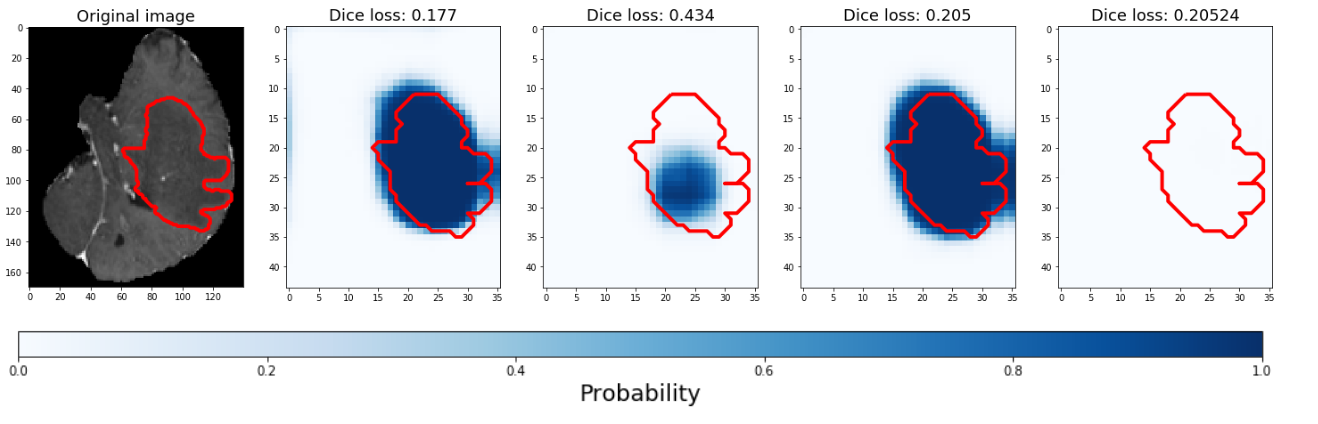
\includegraphics [scale=0.5] {images/series_dice_1.png}

\end{figure}

\begin{figure}[h!] 
  \center
  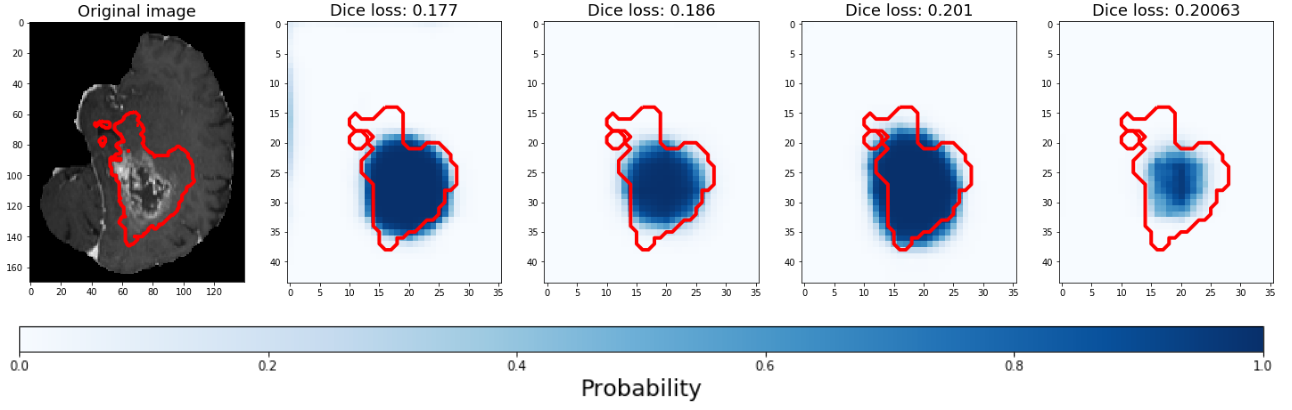
\includegraphics [scale=0.5] {images/series_dice_2.png}

\end{figure}

\begin{figure}[h!] 
  \center
  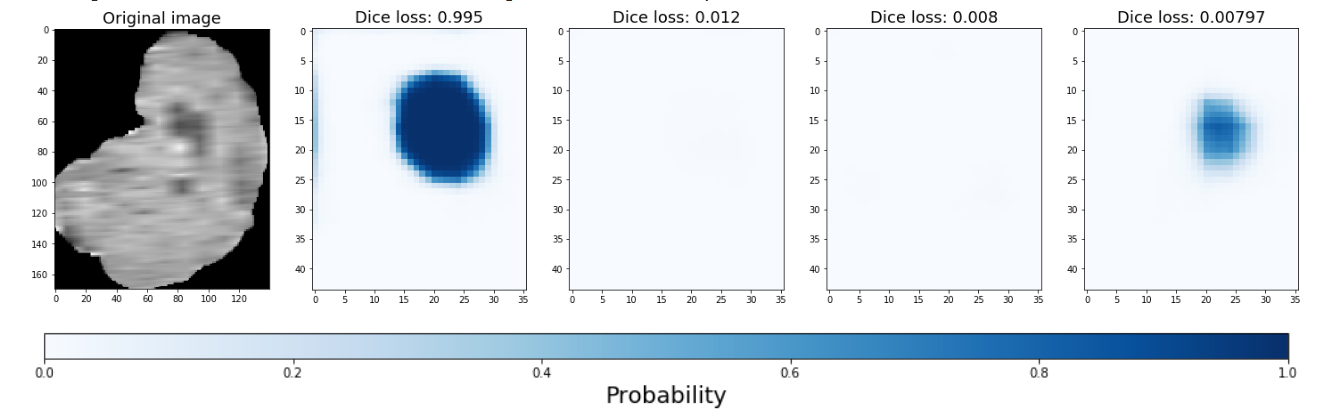
\includegraphics [scale=0.5] {images/series_dice_3.png}

\end{figure}

\begin{figure}[h!] 
  \center
  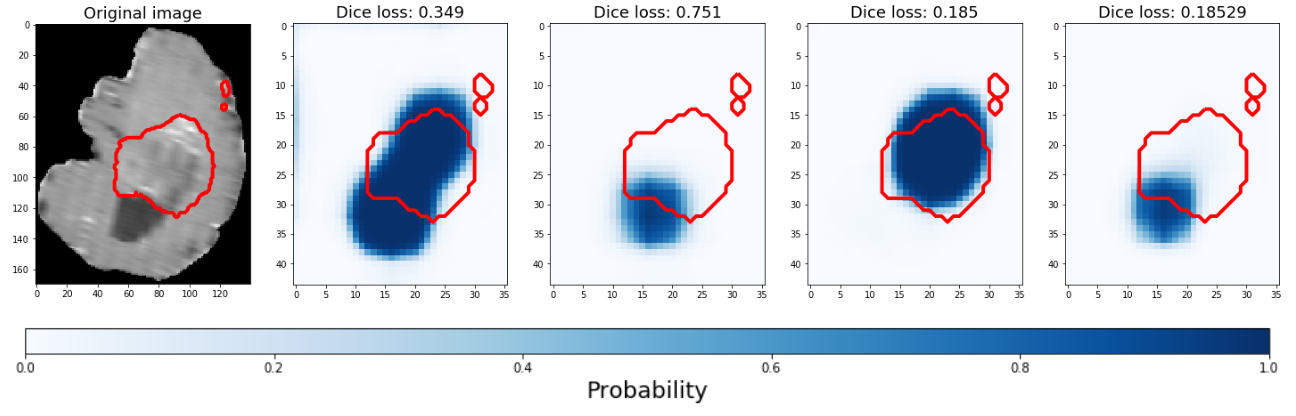
\includegraphics [scale=0.5] {images/series_dice_4.png}

\end{figure}

\begin{figure}[h!] 
  \center
  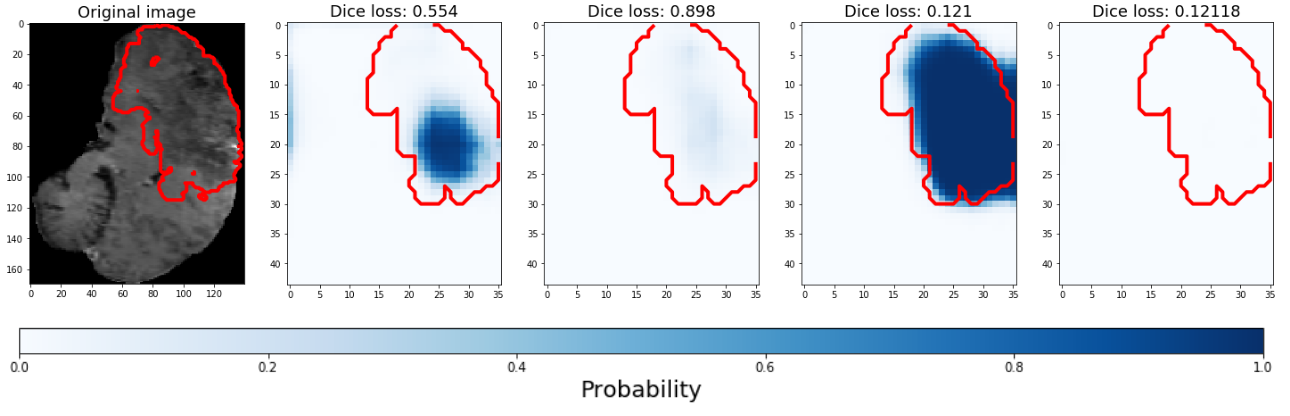
\includegraphics [scale=0.5] {images/series_dice_5.png}

\end{figure}


\begin{figure}[h!] 
  \center
  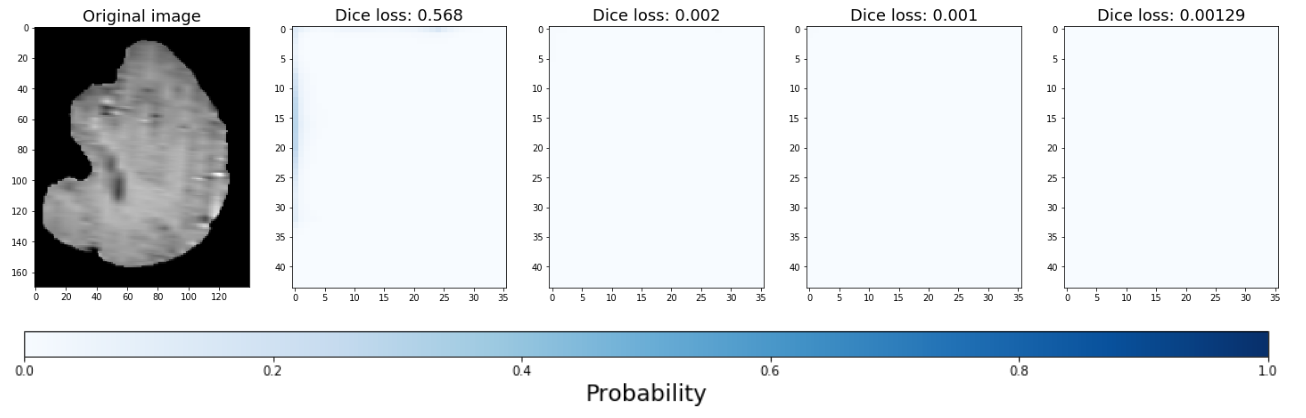
\includegraphics [scale=0.5] {images/series_dice_6.png}

\end{figure}

\newpage
\section{Постановка эксперимента}

Сперва зададимся значением параметра $K = 4$. Будем варьировать следущие факторы:

\begin{itemize}
    \item Функция потерь, на которой происходит обучение в режиме FS: функция потерь Дайса или перекрёстная энтропия;
    \item Размер сильно размеченной выборки. Будем варьировать его следующим образом: 100, 300, 500, 1000, 2000; 
\end{itemize}

\subsubsection{Технические детали}

\noindent Эмпирическим путём был установлен следующий порядок обучения.

\begin{enumerate}

	\item Предобучение на массивном наборе данных ImageNet; в данной работе использована нейросеть ResNet-50 с уже предобученными на ImageNet весами,
	так что данный этап упоминается чисто формально;

	\item Обучение {\bf бинарной классификации}; обучение происходит в режиме Early Stopping 3 epochs(останавливаем процесс обучения, когда 
	нет улучшений потерь на валидационном наборе данных в течение 3 подряд идущих эпох) с сохранением и последующей подгрузкой лучших полученных в процессе обучения весов;
	
	\item Обучение сегментации fully supervised ({\bf FS}) на относительно небольшом наборе данных с сильной разметкой в режиме Early Stopping 5 epochs(аналогично предыдущему, только для 5 подряд идущих 
	эпох обучения);
	
	\item Обучение метода MIL(будем также говорить - fine tuning модели - {\bf FT}) производилось в режиме Early Stopping 1 epoch с толерантностью к улучшению Dice loss, равной 0.01(все меньшие улучшения таковыми не считались);
	
	\item При обучении тренировочная и валидационная выборки балансировались по числу изображений положительного и отрицательного класса(сперва выбиралось возможное число положительных с учётом выборки(1\%, 5\% или 10\%), затем бралось такое же число изображений, не содержащих опухоли, поэтому значения 100, 300, 500, 1000 и 2000 следует воспринимать как {\bf удвоенные} количества изображений с попиксельной разметкой)

\end{enumerate}

При оптимизации использовался метод оптимизации Adam. При этом шаг оптимизации(learning rate) для классификации и FS-обучения выбирался равным $5*10^{-5}$, а для FT-обучения снижался пропорционально размеру сильно размеченного набора данных(эвристика).


\subsection{Результаты эксперимента}

Как было упомянуто выше, необходимо установить, какую функция потерь лучше всего использовать для FS-обучения. 

\noindent В таблицах ниже приведены результаты эксперимента. Читать таблицы следует следущим образом:

\begin{itemize}
    \item По строкам - результаты для этапов 5-перекрёстной валидации;
    \item <<LR>> - шаг обучения;
    \item <<Classifier Acc>> - точность предобученной бинарной классификации;
    \item <<Dice Loss Val FS>> - Dice loss для  FS-обучения, полученный при валидационной выборке - в случае прямого обучения FS на Dice loss и в случае непрямого(LogLoss) соответственно;
    \item <<Dice Loss Val FT>> -  полученный на валидационной выборке итоговый Dice loss для FT-обучения(MIL) над результатом FS-обучения - в случае прямого обучения FS на Dice loss и в случае непрямого(LogLoss) соответственно;
    \item Строка <<AVG>> - среднее по столбцам c доверительными интервалами Стьюдента по пяти значениям кросс-валидации;
    \item Данные в каждой таблице для разделов <<Dice>> и <<Logloss>> посчитаны на одном и том же для данной таблицы разбиении, а значит, позволяют сравнивать метрики между собой.
\end{itemize}

\begin{figure}[h!] 
  \center
  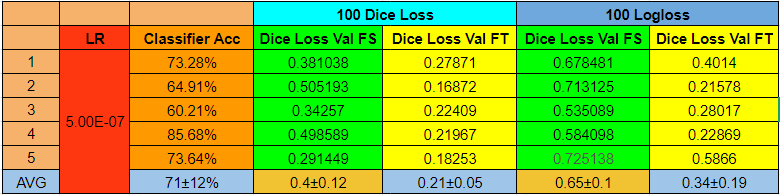
\includegraphics [scale=1.0] {images/experiment_100.png}
  \caption{ Результаты для эксперимента с 50 сильно размеченными изображениями для FS (+50 не содержащих опухоли - итого 100) } 
\end{figure}

\begin{figure}[h!] 
  \center
  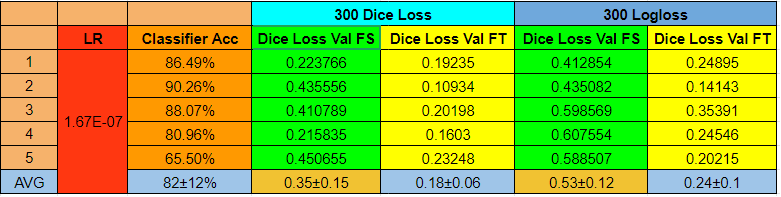
\includegraphics [scale=1.0] {images/experiment_300.png}
  \caption{  Результаты для эксперимента со 150 сильно размеченными изображениями для FS (+150 не содержащих опухоли - итого 300) } 
\end{figure}

\begin{figure}[h!] 
  \center
  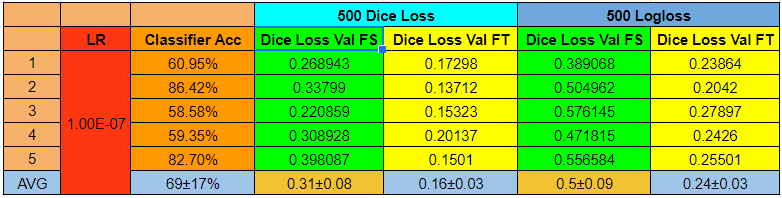
\includegraphics [scale=1.0] {images/experiment_500.png}
  \caption{  Результаты для эксперимента со 250 сильно размеченными изображениями для FS (+250 не содержащих опухоли - итого 500)} 
\end{figure}

\begin{figure}[h!] 
  \center
  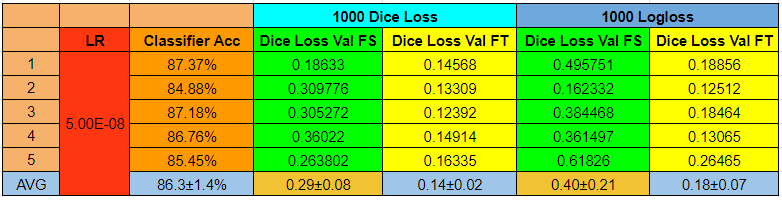
\includegraphics [scale=1.0] {images/experiment_1000.png}
  \caption{  Результаты для эксперимента с 500 сильно размеченными изображениями для FS (+500 не содержащих опухоли - итого 1000)} 
\end{figure}

\begin{figure}[h!] 
  \center
  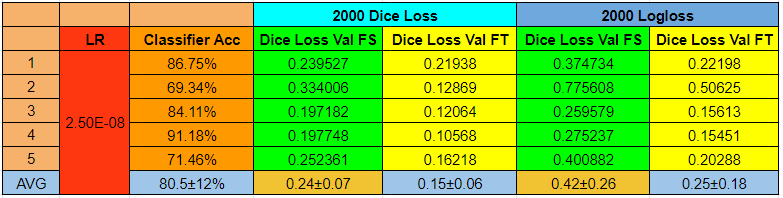
\includegraphics [scale=1.0] {images/experiment_2000.png}
  \caption{  Результаты для эксперимента с 1000 сильно размеченными изображениями для FS (+1000 не содержащих опухоли - итого 2000)} 
\end{figure}

Также дополним полученные таблицы графиком, в котором <<dice-fs>>, <<dice-ft>>, <<log-fs>>, <<log-ft>> соответствуют упомянутым в пояснениях к таблицам выше категориям. 

\begin{figure}[h!] 
  \center
  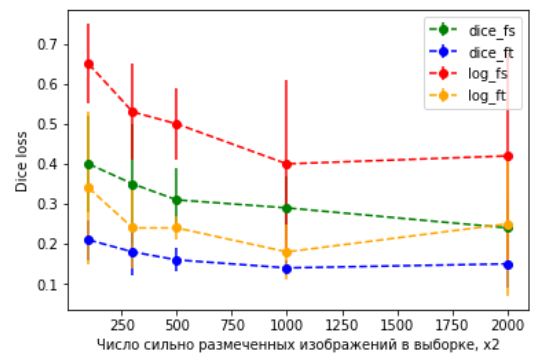
\includegraphics [scale=1.2] {images/plot_results.png}
  \caption{ Результаты эксперимента} 
\end{figure}

{\bf Выводы:} 

\begin{itemize}
    \item из графиков видно, что подход с прямой оптимизацией на Dice loss более предпочтителен с точки зрения итогового индекса Дайса после FT- обучения;
    \item лучший существующий на сегодняшний день результат сегментации, полученный на наборе BRATS2018 равен 0.9\cite{BRATS_winning_2018}; можно заметить, что на упрощённой задаче (<<$\ge$10\%>>) наш метод приближается к этому результату; 
\end{itemize}

\section{Необходимость классификаци}

С тем чтобы установить необходимость предобучения на бинарной классификации, был поставлен следующий эксперимент: для одного и того же разбиения(5-кросс-валидации) было произведено FS - обучение в двух случая:
\begin{itemize}
    \item С предварительным предобучением на задаче бинарной классификации;
    \item Без предварительного предобучения на задаче бинарной классификации;
\end{itemize}



\noindent Приведем пример графиков для $K = 6$ и 1000 сильно размеченных изоображений, демонстрирующих сходимость процессов FS-обучений в обоих случаях(\ref{fig:cmp_class_no_class}).

\begin{figure}[h!] 
  \center
  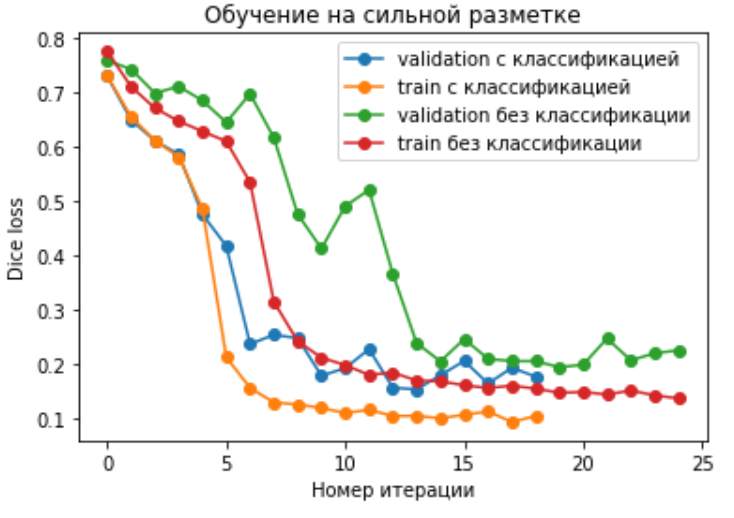
\includegraphics [scale=0.8] {images/cmp_class_no_class.png}
  \caption{ Пример сходимости метода с предобучением на задаче классификации и без} \label{fig:cmp_class_no_class}
\end{figure}

\begin{figure}[ht] 
  \center
  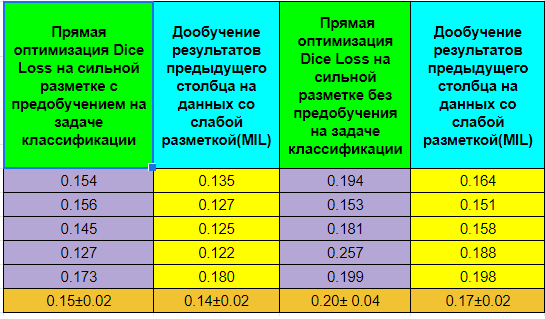
\includegraphics [scale=0.78] {images/shortcut.png}
  \caption{ Сравнение результатов FS и FT для случаев с предобучением на классификации и без} 
  \label{fig:cmp_pretrain}  
\end{figure}

{\bf Выводы:}

\begin{itemize}
    \item Из таблицы  (\ref{fig:cmp_pretrain}) следует, что  предобучение на классификации более предпочтительно;
    \item Из графика видно, что по крайней мере при данных значениях шагов обучения ($5*10^{-6}$ для FS и $10^{-6}$ для MIL) с предобучением на задаче классификации метод сходится быстрее; однако не стоит забывать, что и само предобучение классификации занимает немало времени, в особенности в режиме Early Stopping;

\end{itemize}


\section{Подбор значения параметра К}

Данный параметр будем подбирать в отдельности для каждого из выбранных наборов данных. 

В таблицах ниже приведём результаты 5-кросс-валидации для различных значений параметра K и наборов данных <<10\%>> и <<5\%>>.



\begin{figure}[h!] 
  \center
  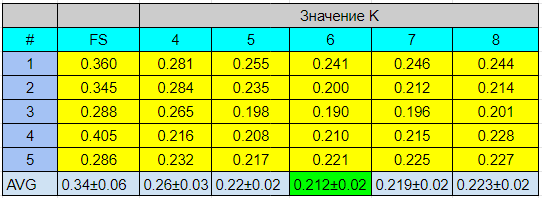
\includegraphics [scale=1.0] {images/5_percent_experience.png}
  \caption{ Выборка данных <<$\ge$ 5\% >>} 
  \label{fig:5_perc}  
\end{figure}


\begin{figure}[h!] 
  \center
  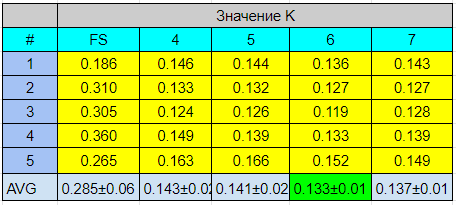
\includegraphics [scale=1.0] {images/10_percent_experience.png}
  \caption{ Выборка данных <<$\ge$ 10\% >>} 
  \label{fig:10_perc}  
\end{figure}

Вопреки ожиданиям, оказалось, что при появлении снимков с малой площадью опухоли, оптимальное значение параметра K не сдвигается в меньшую сторону: значение $K=6$ остаётся оптимальным и при добавлении меньших сегментаций.

\newpage

\section{Обсуждение порядка следования этапов обучения}
По аналогии с вопросом предыдущего параграфа  возникает вопрос:  {\bf можно ли поменять местами FS и FT-этапы} ? И если возможно, то нужно ли использовать предобучение на задаче классификации? Было установлено, что смена порядка этапов чувствительна к значению шагов обучения. Путём подбора были выбраны такие шаги обучения: $5*10^{-6}$ для FS и $10^{-6}$ для MIL. Ниже приведена таблица, демонстрирующая также в режиме кросс-валидации результаты эксперимента для $K = 6$ и 1000 сильно размеченных изображений для различных порядков обучения с предобучением на классификации и без. В таблице также дублируется её часть из предыдущего раздела. Отметим, что значения левой половины отличаются от значений  в \ref{fig:10_perc}, поскольку использовались другие шаги обучения.  Как и в предыдущем параграфе, приведём примеры графиков сходимости методов для случаев с предобучением на классификации и без. Результаты говорят о том, что при использовании метода MIL в начале, необходимо предобучить ResNet-50 на задаче классификации.


\begin{figure}[h!] 
  \center
  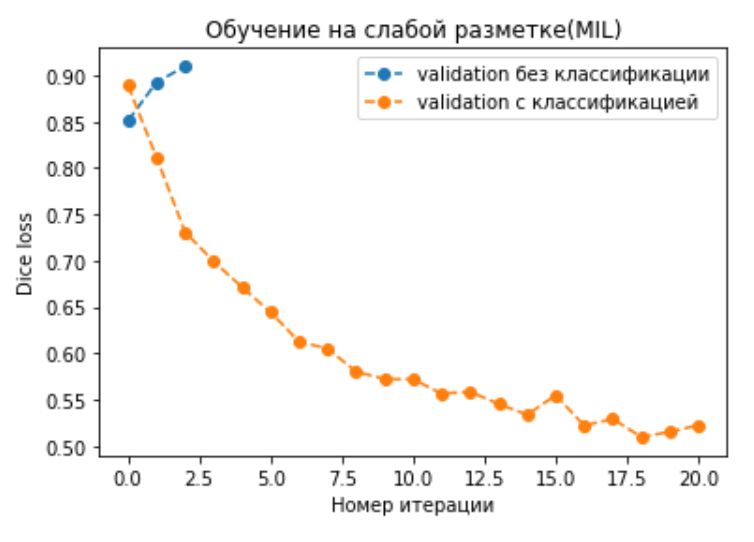
\includegraphics [scale=0.7] {images/cmp_order_mil.png}
  \caption{ Различная сходимость метода MIL(до FS) в зависимости от использования предобучения на классификации }
  \label{fig:mil_order}  
\end{figure}

\begin{figure}[h!] 
  \center
  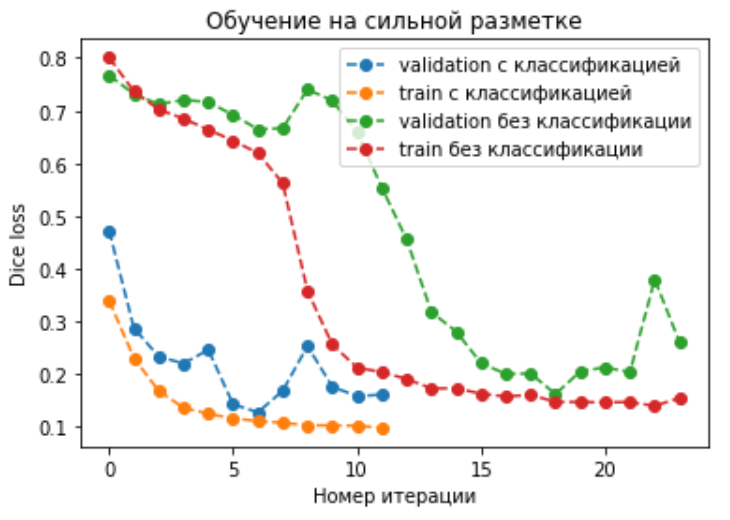
\includegraphics [scale=0.7] {images/cmp_order_class.png}
  \caption{ Различная сходимость метода FS(после MIL) в зависимости от использования предобучения на классификации }
  \label{fig:cmp_order_class}  
\end{figure}


\begin{figure}[h!] 
  \center
  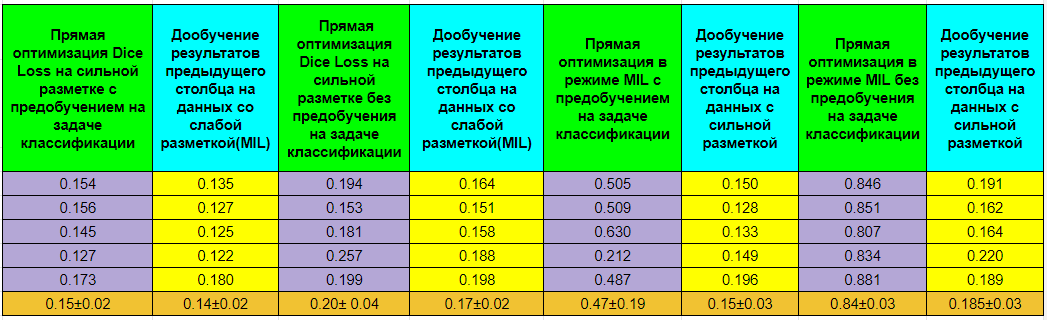
\includegraphics [scale=0.8] {images/total_table_results.png}
  \caption{ Результаты прямого и обращенного порядка обучения этапов FT и FS с предобучением на классификации и без}
  \label{fig:cmp_order_class}  
\end{figure}

\newpage
\section{Сравнение предложенного подхода с обучением сегментации на сильно размеченном наборе данных}

Необходимо убедиться, в какой степени наш метод позволяет приблизиться к результатам, полученным в случае, когда {\bf вся выборка имеет сильную разметку}. Будем обучать нашу архитектуру на разбиении данных в отношении 80\%/20\%(train/validation) для наборов данных <<1\%>>(~21.000 изобрежний), <<5\%>>(~16.000 изображений) и <<10\%>>(~9.000 изображений). На графиках ниже приводятся кривые обучения для каждого из наборов данных, также в таблице \ref{fig:cmp_with_fs} приведено сравнение результатов метода(5-CV, $K=6$, 500(+500) размеченных картинок) с результатами обучения на сильно размеченных наборах данных.

\begin{figure}[ht]
    \center{
        \hfill
        \subcaptionbox[List-of-Figures entry]{10\%\label{fig:strong_10}} {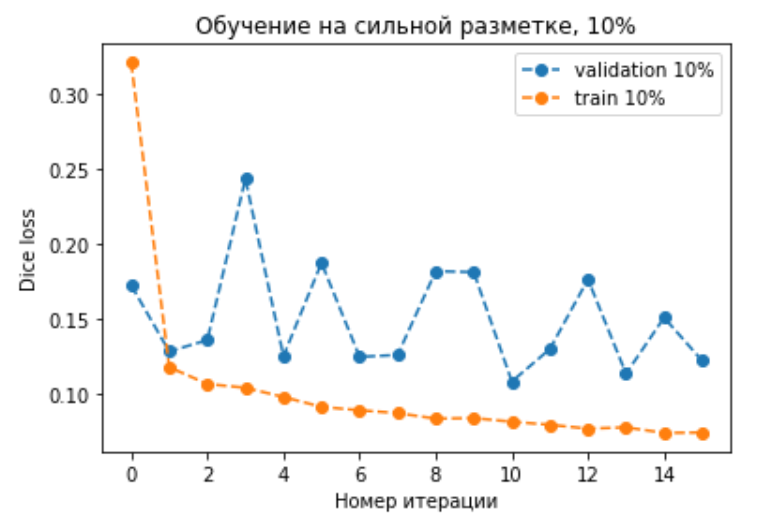
\includegraphics[width=0.5\linewidth]{images/strong_10.png}}%
        \hfill       
        \subcaptionbox{5\%\label{fig:strong_5}} {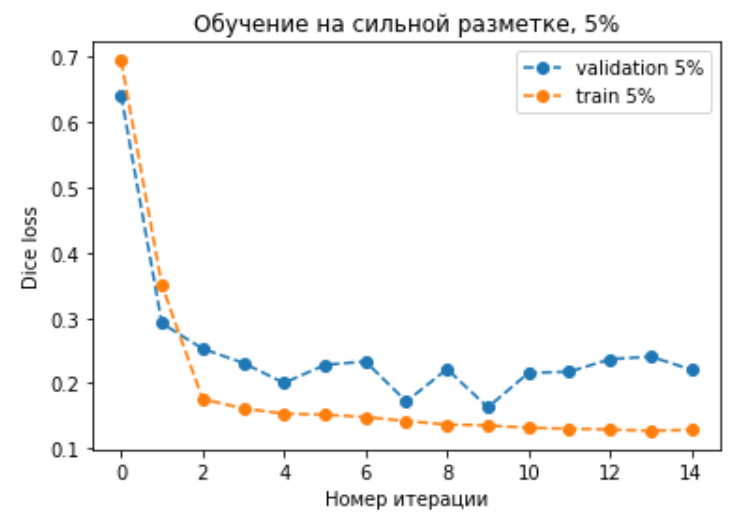
\includegraphics[width=0.5\linewidth]{images/strong_5.png}}
        \hfill
    }
    

    \caption{Кривая обучения для набора данных <<10\%>> и <<5\%>>} % Этот текст попадает в названия рисунков в списке рисунков
    \label{fig:cmp_order_class}  
\end{figure}

\begin{figure}[h!] 
  \center
  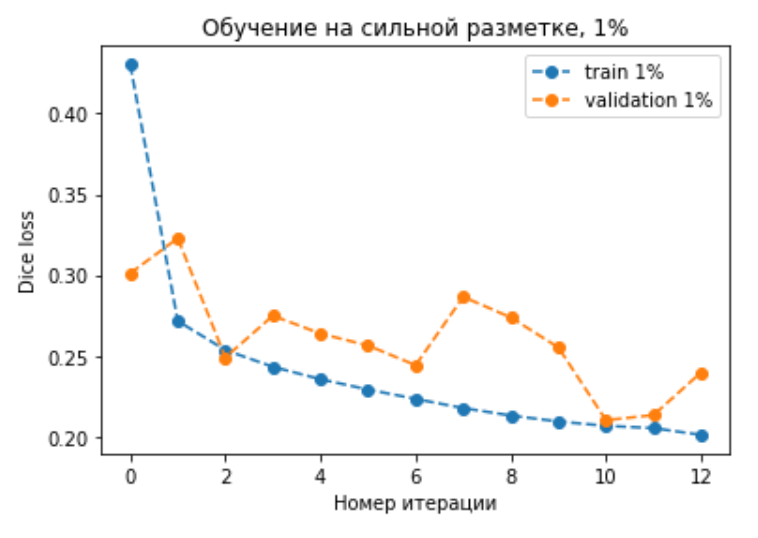
\includegraphics [scale=0.8] {images/strong_1.png}
  \caption{Кривая обучения для набора данных <<1\%>>}
  \label{fig:strong_1}  
\end{figure}

\begin{figure}[h!] 
  \center
  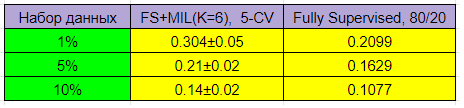
\includegraphics [scale=1.0] {images/compare_with_fs.png}
  \caption{Сравнительная таблица методов}
  \label{fig:cmp_with_fs}  
\end{figure}
\newpage
\subsection{Примеры сегментации}

Приведём несколько примеров сегментаций, демонстрирующих различе работы нашего метода(FS+MIL, 500(+500) изображений с сильной разметкой) и обучения на наборе из 7.000 сильно размеченных изображений(<<Fully supervised>>, <<10\%>>)(рис.\ref{fig:cmp_fs_ours}).   Изображения взяты из общего для моделей валидационного набора. Над каждым примером сегментации подписана величина Dice Loss. Разница в качестве сегментации очевидна, но зачастую она не очень велика. В следующем разделе будет приведено сравнение полученных с помощью нашего метода сегментаций с сегментациями, полученных на обучении на {\bf малом} сильно размеченном наборе({\bf FS}). Можно будет сказать, что наш метод улучшает обучение на малом сильно размеченном наборе, но немного уступает в качестве обучению на полностью сильно размеченном наборе большого размера. 

\begin{figure}[h!] 
  \center
  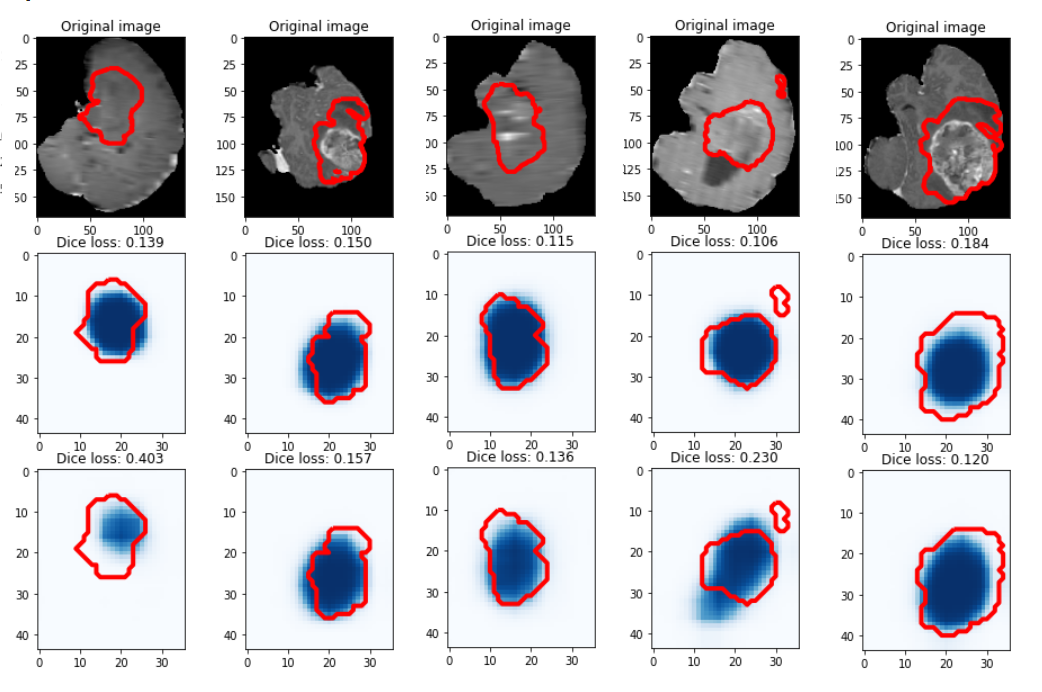
\includegraphics [scale=0.8] {images/cmp_fs_ours.png}
  \caption{Первый ряд: оригинальное изображение с контуром сегментации; Второй ряд: обучение на сильно размеченных данных; Третий ряд: предложенный метод FS+MIL(K=6), 500(+500))}
  \label{fig:cmp_fs_ours}  
\end{figure}




\newpage
\section{Примеры улучшения и ухудшения сегментации}

Приведённые ниже изображения иллюстрируют таблицу \ref{fig:10_perc}: значение K над изображениями указывает, какому значению K в таблице модель соответствует. Методология следующая: берутся {\bf 100 подряд идущих} изображений {\bf валидационной выборки} и отбираются {\bf все}, демонстрирующие визуальное ухудшение или улучшение сегментации относительно FS-обучения на слабо размеченном наборе данных. 

Среди первых {\bf 100} подряд идущих изображений было зафиксировано {\bf 3} случая ухудшения качества сегментации после применения MIL, и {\bf 22 случая} её улучшения. 

\subsection{Ухудшение сегментации}

\begin{figure}[h!] 
  \center
  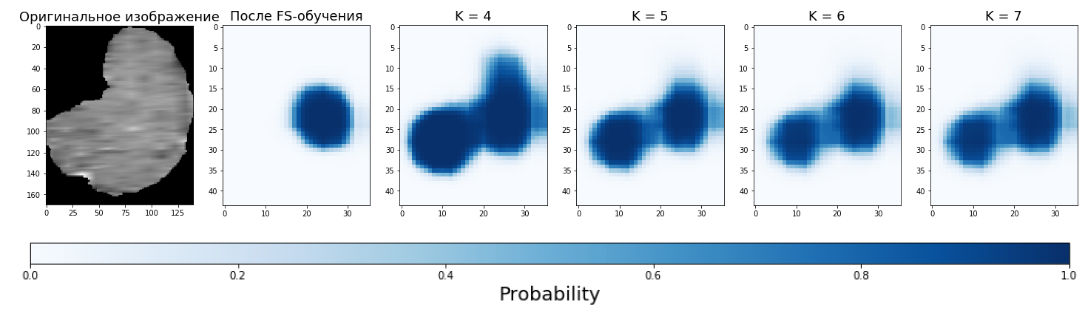
\includegraphics [scale=0.7] {images/bad_1.png}
\end{figure}

\begin{figure}[h!] 
  \center
  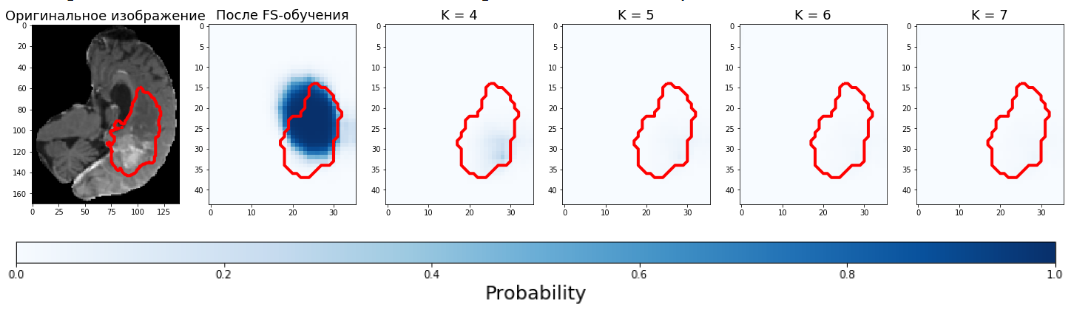
\includegraphics [scale=0.7] {images/bad_2.png}
\end{figure}


\begin{figure}[h!] 
  \center
  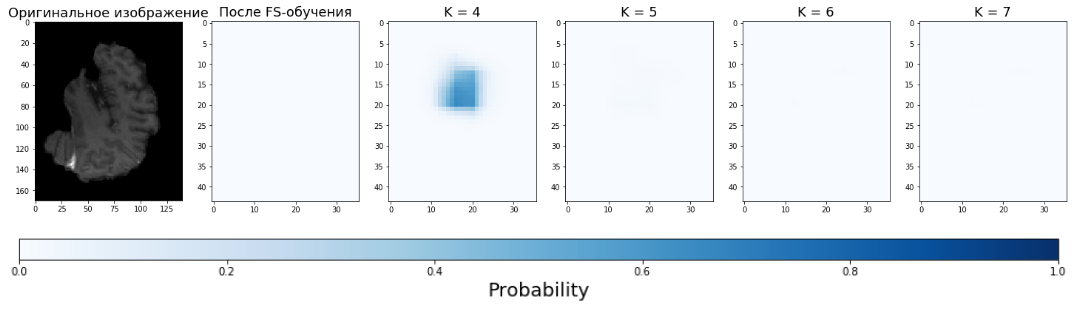
\includegraphics [scale=0.7] {images/bad_3.png}
\end{figure}

\newpage
\subsection{Улучшение сегментации}

\begin{figure}[h!] 
  \center
  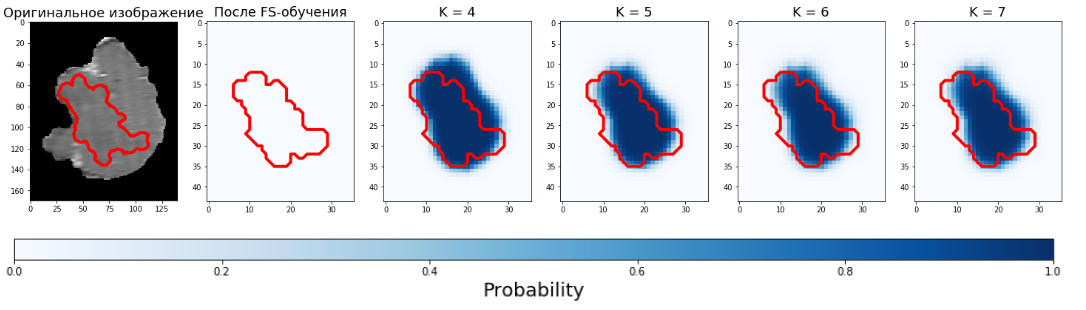
\includegraphics [scale=0.7] {images/good_1.png}
\end{figure}


\begin{figure}[h!] 
  \center
  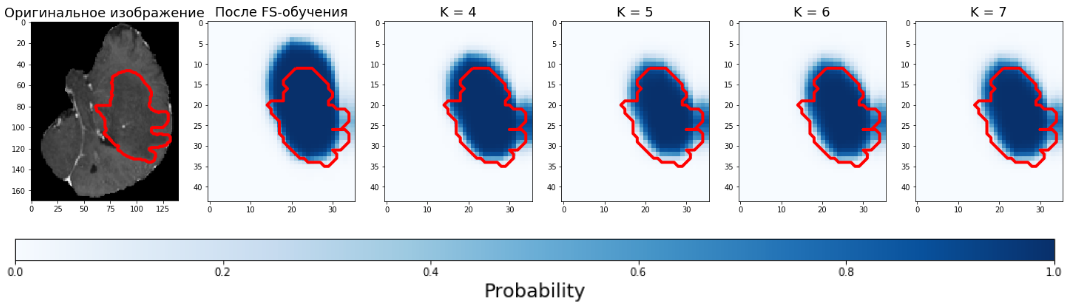
\includegraphics [scale=0.7] {images/good_2.png}
\end{figure}

\begin{figure}[h!] 
  \center
  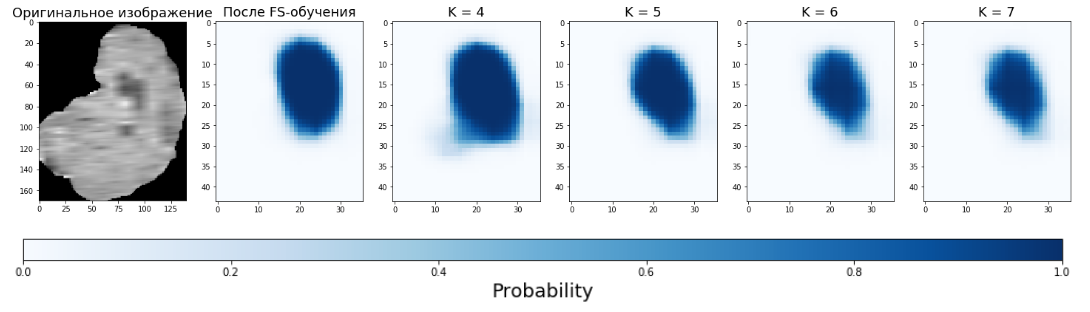
\includegraphics [scale=0.7] {images/good_3.png}
\end{figure}

\begin{figure}[h!] 
  \center
  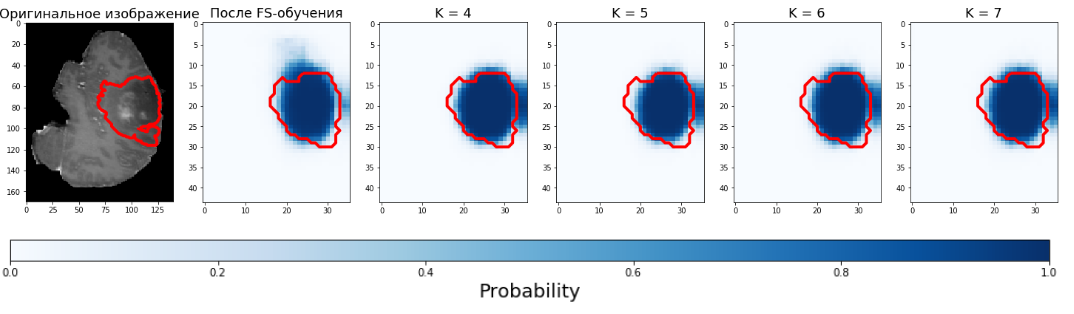
\includegraphics [scale=0.7] {images/good_4.png}
\end{figure}


\begin{figure}[h!] 
  \center
  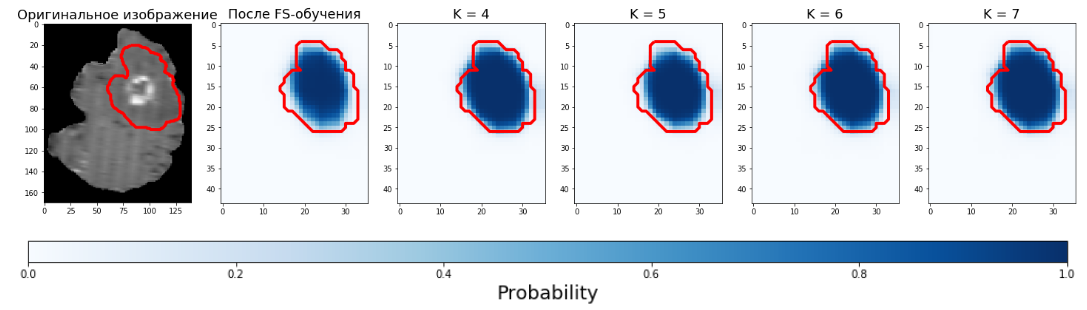
\includegraphics [scale=0.7] {images/good_5.png}
\end{figure}


\begin{figure}[h!] 
  \center
  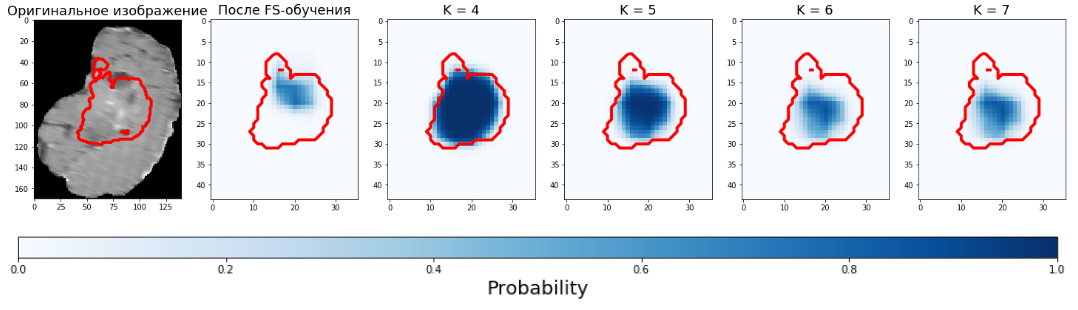
\includegraphics [scale=0.7] {images/good_6.png}
\end{figure}

\begin{figure}[h!] 
  \center
  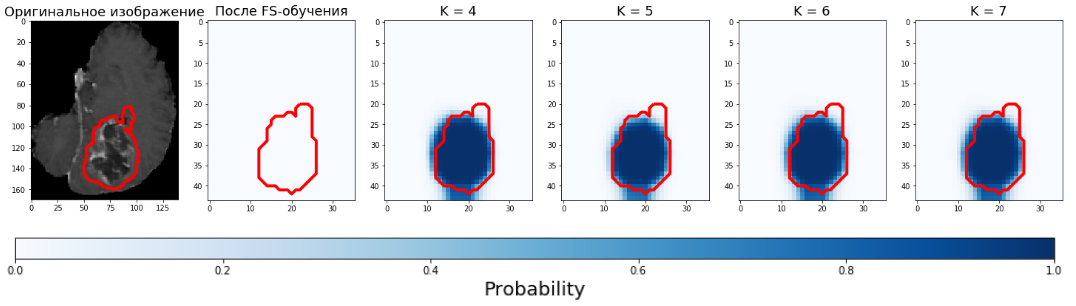
\includegraphics [scale=0.7] {images/good_7.png}
\end{figure}

\begin{figure}[h!] 
  \center
  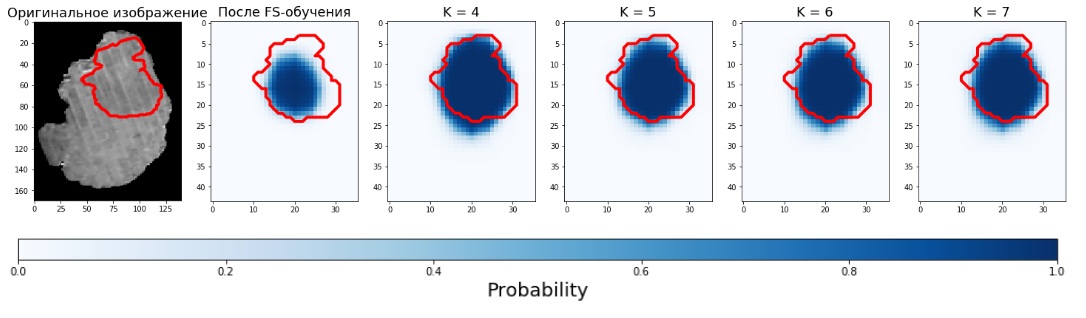
\includegraphics [scale=0.7] {images/good_8.png}
\end{figure}

\begin{figure}[h!] 
  \center
  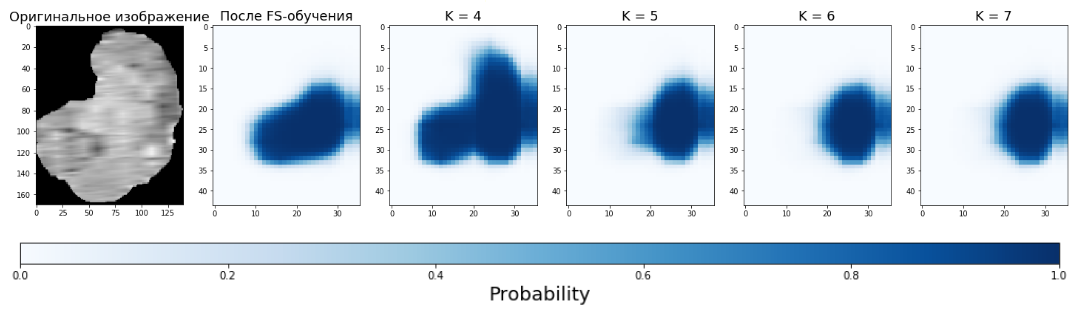
\includegraphics [scale=0.7] {images/good_9.png}
\end{figure}


\begin{figure}[h!] 
  \center
  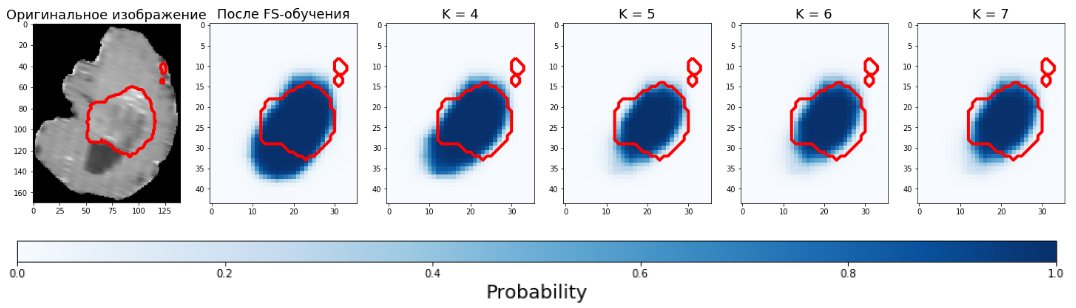
\includegraphics [scale=0.7] {images/good_10.png}
\end{figure}

\begin{figure}[h!] 
  \center
  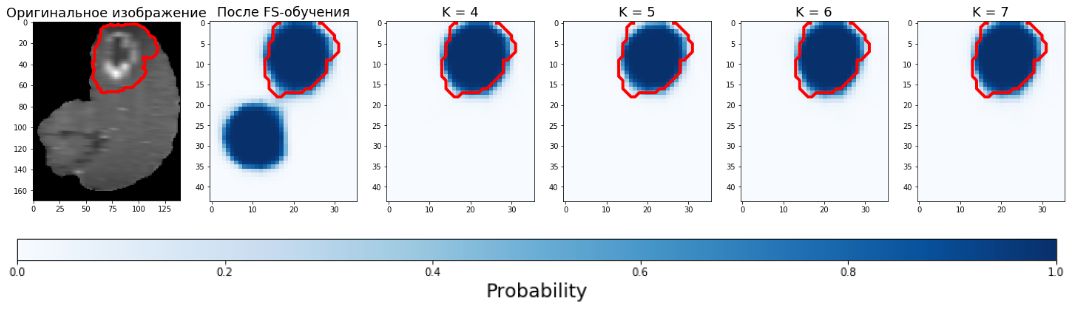
\includegraphics [scale=0.7] {images/good_11.png}
\end{figure}

\begin{figure}[h!] 
  \center
  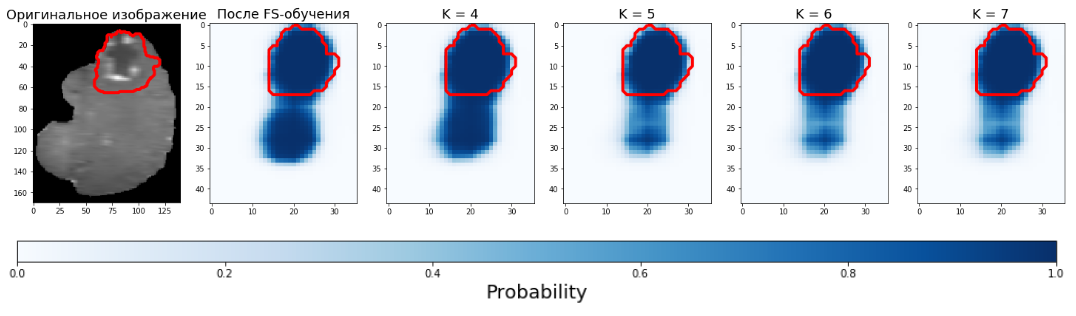
\includegraphics [scale=0.7] {images/good_12.png}
\end{figure}

\begin{figure}[h!] 
  \center
  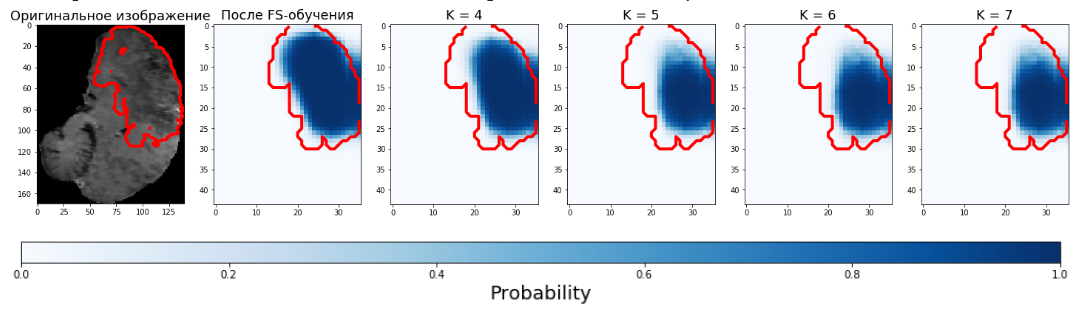
\includegraphics [scale=0.7] {images/good_13.png}
\end{figure}

\begin{figure}[h!] 
  \center
  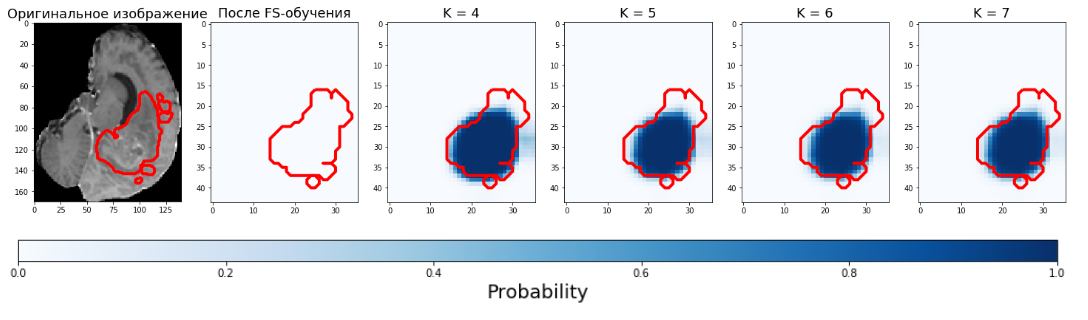
\includegraphics [scale=0.7] {images/good_14.png}
\end{figure}

\begin{figure}[h!] 
  \center
  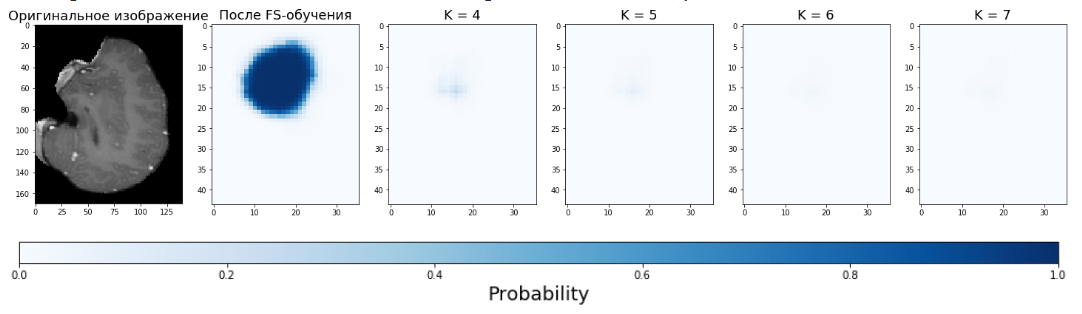
\includegraphics [scale=0.7] {images/good_15.png}
\end{figure}


\begin{figure}[h!] 
  \center
  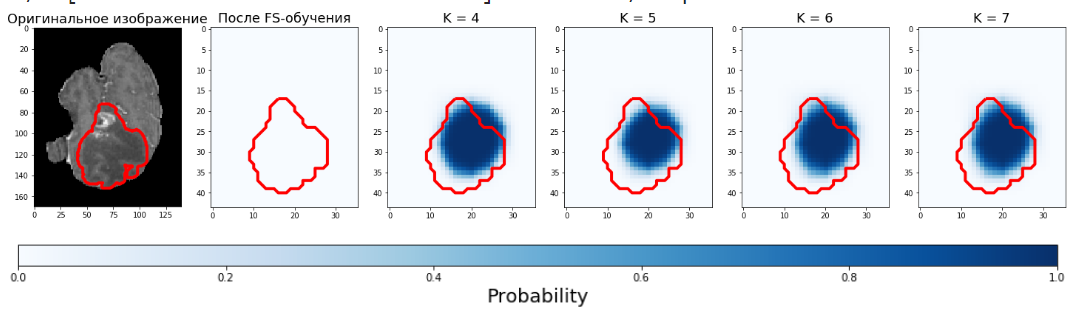
\includegraphics [scale=0.7] {images/good_16.png}
\end{figure}


\begin{figure}[h!] 
  \center
  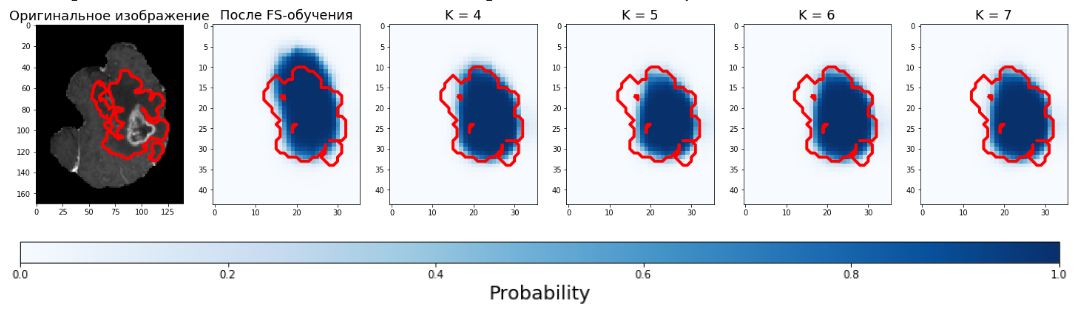
\includegraphics [scale=0.7] {images/good_17.png}
 \end{figure} 
  
  \begin{figure}[h!] 
  \center
  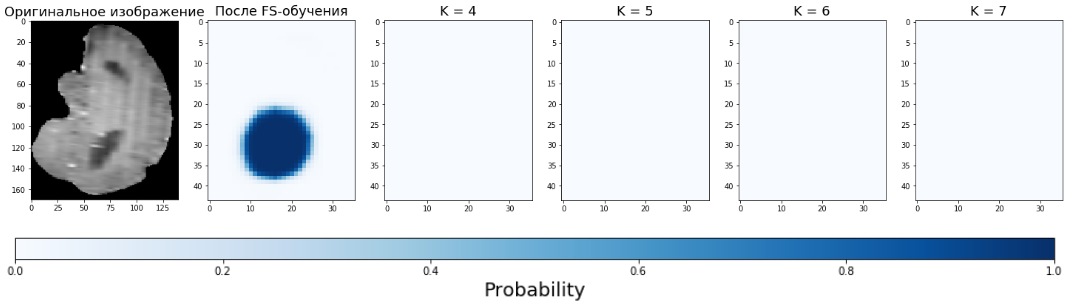
\includegraphics [scale=0.7] {images/good_18.png}
  \end{figure} 
  
  \begin{figure}[h!] 
  \center
  \includegraphics [scale=0.7] {images/good_19.png}
\end{figure}


  \begin{figure}[h!] 
  \center
  \includegraphics [scale=0.7] {images/good_20.png}
\end{figure}

  \begin{figure}[h!] 
  \center
  \includegraphics [scale=0.7] {images/good_21.png}
  \end{figure} 
  
  \begin{figure}[h!] 
  \center
  \includegraphics [scale=0.7] {images/good_22.png}
\end{figure}



\clearpage